\documentclass[a4paper,10pt]{article}
\usepackage[utf8]{inputenc}
\usepackage[UKenglish]{babel}
\usepackage{fancyhdr}
\usepackage{anysize}
\usepackage{amsmath,amssymb,amsfonts,amsthm} % Typical maths resource packages
\usepackage{lastpage}
\usepackage[all]{xy}  % drawings
%\usepackage{listings} % code highlighting
\usepackage[usenames,dvipsnames]{color}
\usepackage{graphicx}
\usepackage{caption}
\usepackage{subfigure}
\usepackage{upgreek}

\pagestyle{fancy}
\fancyfoot[R]{\em \thepage / \pageref{LastPage}}
\fancyfoot[C]{}
\fancyfoot[L]{\em Master VIBOT}
\fancyhead[R]{\em Lab4 - EKF Map Based Localization}
\fancyhead[C]{}
\fancyhead[L]{\em Probabilistic Robotics}
\renewcommand{\headrulewidth}{0.4pt}
\renewcommand{\footrulewidth}{0.4pt}

%\,	 a small space
%\:	 a medium space
%\;	 a large space
%\quad	 a really large space
%\qquad	 a huge space
%\!	 a negative space (moves things back to the left)
        
\begin{document}

\marginsize{2cm}{2cm}{2cm}{2cm}

% Title
%\hspace{1mm}
\begin{center}
\Large \textbf{Lab4 - EKF Map Based Localization}
\end{center}
%\hspace{1mm}

\section{Introduction}

The goal of this Lab exercise is to program an EKF Map Based Localization algorithm to work with data taken from a real Turtlebot.

Map based localization is a concept that in real life each one of us uses whenever we go to a new place. Whenever a human being goes to a new environment it tries to know where he is. In order to do that, what he does is to read a map of the location and try to relate key parts of the environment he has seen with features of the map so he can localize himself in the map while he is moving around. This can be applied also to robots using an EKF map based algorithm:

\begin{center}
	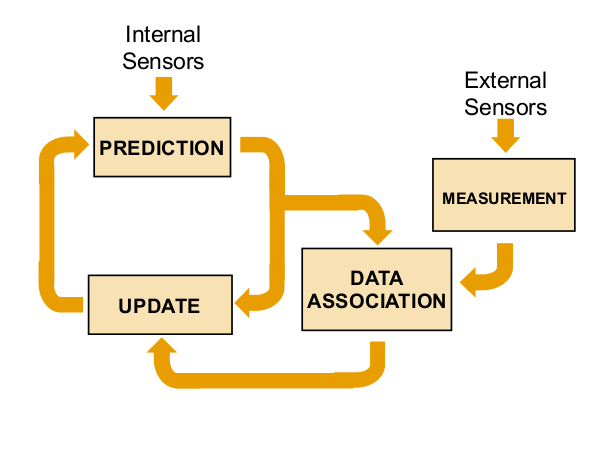
\includegraphics[width=0.50\textwidth]{pict/ekf_pic.png}
	\captionof{figure}{Schematic of EKF map based localization}
	\label{measur}
\end{center}

This EKF map based localization is based in two different sensors, one for the prediction, and one for the update. The prediction is based on the internal odometry of the Turtlebot while the update is based on lines sensed by its Kinect.

\section{Pre-lab}

Read and understand the guide for this Lab and look about the EKF algorithm in your lecture slides.
Find the expressions to compute $x_{k|k-1}^w $ and matrices $A_k$ $W_k$ in order to compute $ P_{k|k-1}^w$ from $x_{k-1}^w$ , $u_k^{r_{k-1}}$ and $Q_k$.
You can write them in paper and attach a picture in the online form submission.

\section{Lab work}

The ROS package named \texttt{ekf\_localization} contains all necessary code for running this lab and a bagfile obtained from a turtlebot with \texttt{nav\_msgs/Odometry} and \texttt{sensor\_msgs/LaserScan} messages. You need to copy your \texttt{splitandmerge.py} solution into the \texttt{src} folder. Then you can test the code by copying the ROS package into your workspace and running

\begin{verbatim}
    roslaunch ekf_localization ekf_localization.launch
\end{verbatim}

As you can see in Rviz that the robot doesn't move at all. You will need to complete the code inside the \texttt{ekf\_localization.py} file in order to complete properly the EKF Localization algorithm. No changes are needed in the \texttt{node.py} nor the \texttt{functions.py} files. If you think you need to modify any of these files ask your lab assistant first.


The EKF algorithm is as follows:

\begin{align*} \scriptsize
    & \blacktriangleright \textit{\textbf{Pose initialization}}\\
    & x_0^w = \hat{x}_0^w \\
    & P_0^w = \hat{P}_0^w \\
    & \textbf{for } \text{k} = 1 \textbf{ to } steps \textbf{ do:} \\
    & \qquad \left[ u_k^{R_{k-1}}, Q_k \right] = get\_odometry() \\
    & \qquad \blacktriangleright \textit{\textbf{EKF prediction}}\\
    & \qquad \left[ x_{k|k-1}^w, P_{k|k-1}^w \right] = move\_vehicle(x_{k-1}^w, P_{k-1}^w, u_k^{R_{k-1}}, Q_k) \\
    & \qquad \left[ z_k, R_k \right] = get\_measurements() \\
    & \qquad \blacktriangleright \textit{\textbf{Data association}}\\
    & \qquad \mathcal{H}_k = data\_association(x_{k|k-1}^w, P_{k|k-1}^w, z_k, R_k) \\
    & \qquad \blacktriangleright \textit{\textbf{EKF update}}\\
    & \qquad \left[ x_k^w, P_k^w \right] = update\_position(x_{k|k-1}^w, P_{k|k-1}^w, z_k, R_k) \\
    & \textbf{end for}
\end{align*}

\subsection{Pose initialization}
The pose initialization is already implemented as:

\begin{align}
    \label{x_0}
    x_0^w &= \begin{pmatrix}
        x_{x_0}\\x_{y_0}\\x_{\theta_0}
    \end{pmatrix} = \begin{pmatrix}
        0.0\\0.3\\-0.03
    \end{pmatrix}\\
    \label{P_0}
    P_0^w &= \begin{pmatrix}
    1 & 0 & 0 \\0 & 1 & 0 \\0 & 0 & 1 
    \end{pmatrix}
\end{align}

\subsection{EKF prediction}

You will need to complete the function \texttt{predict} inside \texttt{ekf\_localization.py}.

This part of the algorithm is where, from the odometry $U_k$ and the previous position the new one is computed. 

\begin{align*}
    & \blacktriangleright \textit{\textbf{Prediction}}\\
    & x_{k|k-1}^w = f(x_{k-1}^w ,u_k^{r_{k-1}}, w_k) \\
    & P_{k|k-1}^w = A_k P_{k-1}^w A_k^T + W_k Q_k W_k^T\\
\end{align*}

These measurements have an uncertainty associated. This uncertainty has been estimated to be 0.025 m as linear noise and 2 degrees as angular noise, so the $Q_k$ matrix can be estimated for all the measurements as:
\begin{align}
    \label{q_k}
    Q_k &= \begin{pmatrix}
	    0.025 & 0 & 0\\0 & 0.025 & 0\\ 0 & 0 & 2
	\end{pmatrix}
\end{align}

Once implemented correctly, when you test the script you should see the robot (blue arrow) moving around the room, and an ellipse representing uncertainty increasing its size when the robot moves.

\begin{center}
	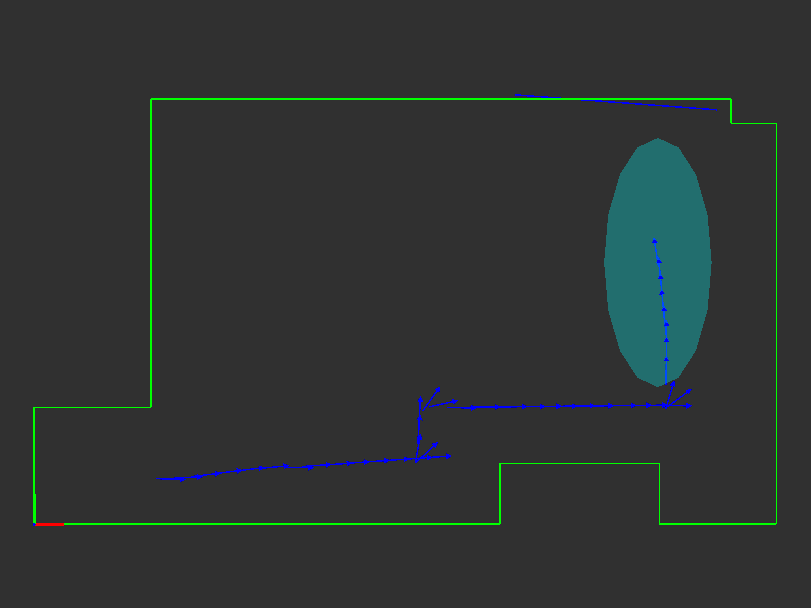
\includegraphics[width=0.70\textwidth]{pict/uncert.png}
	\captionof{figure}{Prediction without updates.}
	\label{no_updates}
\end{center}


\subsection{Data association}

Data association is one of the main parts in the algorithm as it is where it is decided how the position of the robot will be updated, and consequently, whether or not the robot will be positioned in its real position. The aim of this function is to give a list containing to which feature each observation corresponds.
To decide whether or not the distance between a feature and an observation is close enough to claim they are the same, both uncertainties have to be taken into account. To do so, Mahalanobis distance is used.

After computing the distance, the smallest one is chosen, and if it is smaller than a threshold, the observation and the feature are associated. The square of a Gaussian follows a $\upchi_{\rho,\varphi}^2$ distribution, so the threshold will be extracted from there. You will need to choose this threshold value.
\begin{align*}
    & \blacktriangleright \textit{\textbf{Data association}}\\
    & v_{ij} = z_i - h(x_{k|k-1}^w) \\
    & S_{ij} = H_j P_{k|k-1}^w H_j^T + R_i \\
    & D_{ij}^2 = v_{ij}^T S_{ij}^{-1} v_{ij} \\
    & \text{Take the smallest } D_{ij}^2 \text{ if } D_{ij}^2 < \upchi_{\rho,\varphi}^2
\end{align*}

To obtain the measurement function $h(x_{k|k-1}^w)$ that transforms a feature from the real map in polar coordinates in the world frame $x_f^w$ to a feature in polar coordinates in the robot frame $x_f^r$ you can use  Fig.~\ref{measur}.
\begin{center}
	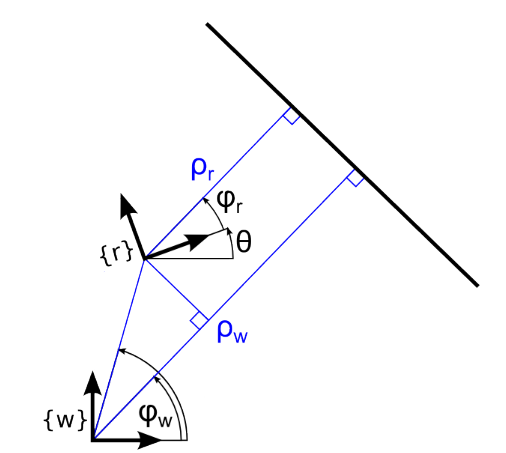
\includegraphics[width=0.50\textwidth]{pict/find_h.png}
	\captionof{figure}{Schematic to deduce the measurement function $h(\hat{x}_{k|k-1}^w)$}
	\label{measur}
\end{center}

Regarding $R_k$, the covariance matrix for the observations, the angle measurement noise has been estimated to 10 degrees and the range measurement to 0.2 m. $R_k$ matrix is estimated as constant.
\begin{align}
    \label{R_k}
    R_k &= \begin{pmatrix}
        0.2 & 0 \\
        0 & 10
    \end{pmatrix}
\end{align}

\subsection{Update}

In this step, the matches obtained on the data association are used to update the position of the robot and its uncertainty. The main algorithm is the following one. Starting by calculating the innovation $v_k$ which is the difference between the observed features $z_k$ and the predicted observation $h(x_{k|k-1}^w)$. Then the uncertainty of this innovation is calculated in $S_k$. Finally. the Kalman gain $K_k$ is computed allowing to update the state vector $x_k^w$ and the covariance matrix $P_k^w$.
\begin{align*}
    & \blacktriangleright \textit{\textbf{Update}}\\
    & v_k = z_k - h(x_{k|k-1}^w) \\
    & S_k = H_k P_{k|k-1}^w H_k^T + R_k \\
    & K_k = P_{k|k-1}^w  H_k^T S_k^{-1} \\
    & x_k^w = x_{k|k-1}^w + K_k v_k \\      
    & P_k = \left( I - K_k H_{k} \right) P_{k|k-1}^w \left( I - K_k H_{k} \right)^T + K_k R_k K_k^T
\end{align*}

Note that $h(x_{k|k-1}^w)$ and $H_k$ have already been computed for each feature in the data association. In this step the difference is that both can have more than one observation to update the robot position. In order to update with all the information at the same time $h(x_{k|k-1}^w)$ and $H_j$ computed for each observation associated to a feature are stacked vertically to obtain the final $h(x_{k|k-1}^w)$ and $H_k$ matrix and be able to run the update algorithm.

\begin{center}
	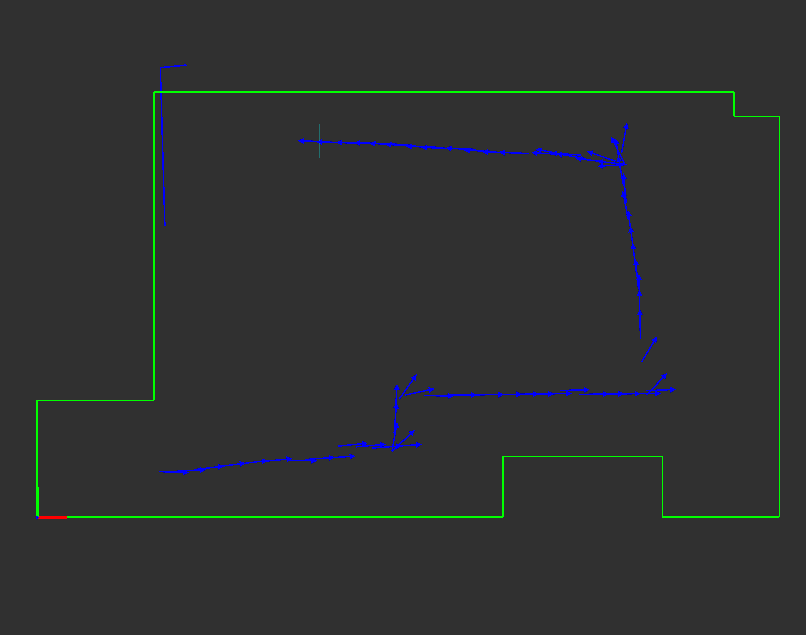
\includegraphics[width=0.70\textwidth]{pict/updates.png}
	\captionof{figure}{Prediction with updates.}
	\label{updates}
\end{center}

\section{Optional}

Using polar representation introduces a new challenge. Walls are represented by lines without ends and not by segments. These can introduce confusions in the data association. Try adding new constraints in the data association subsection to avoid matching the sensed lines with "ghost" walls.

\section{Lab report}

Write a brief report (MAX 4 PAGES) explaining your solution and problems faced. Include the final code.

\end{document}
